\section{型}
プログラミングで使われるデータには「型」と呼ばれるものがある.例えば1や2は「数値」で``Hello''というテキストは「文字列」という型である.Pythonには様々なデータ型が用意されている.今回はその中でも重要な数値,文字列,Bool,リストについて説明する.
\subsection{数値型}
CやJavaでは「整数」と「小数」は別物であり,表現できる上限値が決まっている.Javaの整数型であるintは整数を表現する型であるため,小数点は扱うことができない.Pythonでも正確には整数型や小数型は存在するものの,それらは同じ「数値型」のようなイメージで扱うことが出来る.
数値計算では表\ref{arithmetic_operator}の演算子が利用可能である.

\begin{table}[h]
\centering
 \caption{算術演算子}
  \begin{tabular}{|c|c|} \hline
    操作 & 結果  \\ \hline \hline
    x + y & xとyの和 \\ \hline
    x - y & xとyの差 \\ \hline
    x * y & xとyの積 \\ \hline
    x / y & x割るyの商 \\ \hline
    x \% y & x割るyの余剰 \\ \hline
    x ** y & xのy乗 \\ \hline
    x // y & 切り捨て除算 \\ \hline
  \end{tabular} 
 \label{arithmetic_operator}
\end{table}

\subsection{文字列型}
文字列はシングルクォーテーション(')かダブルクォーテーション(")で囲む.テキストも数値と同様に(+)を使った結合や(*)による繰り返しが出来る.またクォート記号三つで複数行に分けて書くことや[n]でn番目の文字を取り出すことが可能である (ソースコード\ref{str}).
\begin{lstlisting}[caption=文字列の操作, label=str]
>>> s = "str"
>>> print s[1] # 「t」が表示される
>>> print 'abc' + 'def' # 「abcdef」が表示される
>>> print "YO" * 5 #「YOYOYOYOYO」が表示される 
>>> print """HE
... LL
... O!
... """
「HE
  LL
  O!」が表示される
\end{lstlisting}

\subsection{Bool型}
Boolは「真偽値」とも呼ばれる「True/False」の二値を持つ型である.Boolは表\ref{comparative_operator}に示した比較演算子と呼ばれる記号で二つの値を比較した際に返される.
\begin{table}[htbp]
 \centering
   \caption{比較演算子}
    \begin{tabular}{|c|c|} \hline
     操作 & 意味 \\ \hline \hline
     x == y & xとyは等しい \\ \hline
     x is y & xとyは同一のオブジェクト \\ \hline
     x != y & xとyは等しくない \\ \hline
     x is not y & xとyは同一のオブジェクトではない \\ \hline
     x \textgreater y & xはyより小さい \\ \hline
     x \textless y & xはyより大きい \\ \hline
     x \textgreater= y & xはy以下 \\ \hline
     x \textless= y & xはy以上 \\ \hline
     x in y & xの要素がyに含まれる \\ \hline
     x not in y & xの要素がyに含まれない \\ \hline
    \end{tabular}
   \label{comparative_operator}
\end{table}

また,複数の比較演算子の結果を組み合わせて評価する場合,表\ref{logical_operator}の論理演算子を用いる.
\begin{table}[htbp]
 \centering
  \caption{論理演算子}
   \begin{tabular}{|c|c|} \hline
   操作 & 意味 \\ \hline \hline
   not x & xが偽であれば真 \\ \hline
   x and y & xもyも真ならば真 \\ \hline
   x or y & xまたはyが真ならば真 \\ \hline
   \end{tabular}
  \label{logical_operator}
\end{table}

%>>> not 10 < 5
%True
%>>> 10 == 10 and 5 == 5
%True
%>>> 10 < 5 or 10 > 5
%True

\subsection{リスト}
リスト型はデータを「リスト」状に複数個並べたような型である.リストを使わずに3人の学生の平均点を求めようとすると以下のようになる(ソースコード\ref{unused_list}).
\begin{lstlisting}[caption=リストを使わない場合, label=unused_list]
>>> student1 = 68
>>> student2 = 81
>>> student3 = 49
>>> average = (student1 + student2 + student3) / 3
>>> print average
\end{lstlisting}
ソースコード\ref{unused_list}の場合,学生の人数が4人になった場合,修正する箇所が多いことが問題点としてあげられる.このような問題はリストを使うことである程度解消することが出来る.リストは「リストというデータの中に複数のデータを格納できる」という型なので,「学生達の点数」というデータに「具体的な各学生の点数」を格納する.
\begin{lstlisting}[caption=リストを使った場合, label=list1]
>>> results = [68, 81, 49]
>>> average = sum(results) / len(results)
>>> print average
\end{lstlisting}
ソースコード\ref{list1}の1行目で「学生たちの点数」というリストを作成している.2行目にあるsum()はリスト内にあるデータの合計値を算出する関数,len()はリストに格納される要素数を返す関数である.学生一人ひとりの点数毎に変数を作成していないので,「複数の学生たちの点数の格納」が簡単なことに加え,平均値の算出方法が学生の数に依存していない.リストを使うことで「ひとつのグループに属するデータ」を便利に扱うことが出来る.
\begin{lstlisting}[caption=リストの使い方1, label=list2]
>>> a = []
>>> b = [1, 2, 3]
>>> c = [1, "2", False]
\end{lstlisting}
ソースコード\ref{list2}の1行目のように,[]の中に何も入れない場合は空のリストを作成する.3行目のようにリストの中に様々なデータが入れられることには注意したい.リストの要素を取り出すにはリスト内のx番目の要素を指定する必要がある.また,指定する順序は1からではなく0からである(ソースコード\ref{list3}).
\begin{lstlisting}[caption=リストの使い方2, label=list3]
リスト名[要素の番号]

>>> b = [1,2,3]
>>> print(b[0]) # 1
>>> print(b[2]) # 3
>>> b[1] = 5
>>> print(b[1]) # 5
>>> b.append(4)   # 末尾へ4を挿入
>>> print(b)
[1, 5, 3, 4]
>>> b.insert(1,10)   # 1番目の要素に10を挿入
>>> print(b)
[1, 10, 5, 3, 4]
>>> b.remove(1)
>>> print(b)
[10, 5, 3, 4]
\end{lstlisting}


\section{ブロックとインデント}
ブロックとは,複数個の文などのコードのまとまりのことである.if文やfor文,関数定義やクラス定義などを利用する際は,ブロックの中に処理を記述することになる.

C言語やJavaが中括弧を用いて処理のブロックを表すのに対して,Pythonはインデント(行頭の空白文字の数)で処理のブロックを表す.コロンで終わる行がブロックの始まりを表し、それ以下のインデントが同じ行を同じブロックと見なす.インデントの空白文字の数は任意であるが,一般的に四つが推奨されている.

\begin{lstlisting}[caption=インデント,label=indent]
>>> x = 3 
>>> if x == 3: #変数xが3である場合,if文以下のブロックを実行する
...     print "AAA" #インデント(スペース4つ)の後に,命令を記述
...     print "BBB" 
... #if文を抜けるために,Enter
AAA #if文の条件が真だったため,if文以下のブロックが実行される
BBB

>>> if x == 5: 
...     print "AAA" 
...     print "BBB"
...
>>> #if文の条件が偽だったため,if文以下のブロックは実行されない
\end{lstlisting}


\section{分岐処理}
ifを使うことで条件に応じた分岐処理を行うことが可能である.ifに続く式が真であればインデントされたブロックの処理が実行される.インデントとはスペースやタブで字下げすることをいう.また,同じインデント幅で揃えられた部分をブロックという.複数の条件を指定する場合elifを用いる.elifは任意の数繰り返すことが可能である.いずれにも該当しない場合の処理はelseに続けて書くが,省略することも出来る.Bool型が条件判定に利用され,その値がTrueかFalseかで実行するプログラムが変わる(ソースコード\ref{if}).
\begin{figure}[htbp]
 \centering
  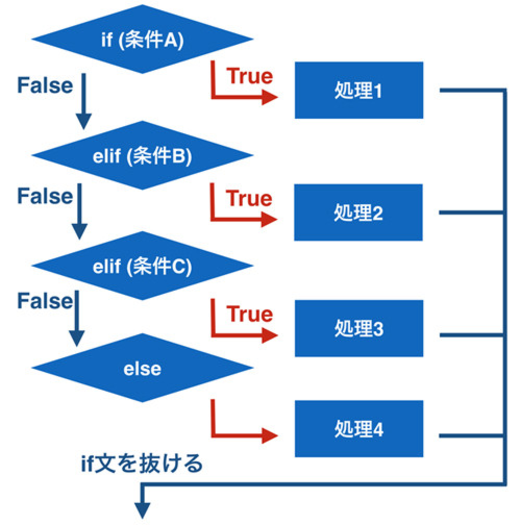
\includegraphics[width=10cm]{001.pdf}
  \caption{条件分岐の仕組み}
\end{figure}
\begin{lstlisting}[caption=ifの使い方,label=if]
if 条件A:
    処理1  # 条件 A が True の時に実行される処理
elif 条件B:
    処理2  # 条件 A が False で条件 B が True の時に実行される処理
elif 条件C:
    処理3  # 条件 A,B が False で条件 C が True の時に実行される処理
else:
    処理4  # 全ての条件が False の時に実行される処理
\end{lstlisting}
%標準入力を用いて入力した値が偶数か奇数かを判定するプログラムを作ってもらう?

\section{ループ処理}
ループ処理は「同じ処理を何度も繰り返す」という処理である.ループ処理の制御構造にはforとwhileの二つがある.
\subsection{while}
whileは条件が真である間,インデントされたブロックの処理を繰り返し実行する(ソースコード\ref{while}).
\begin{figure}[htbp]
 \centering
  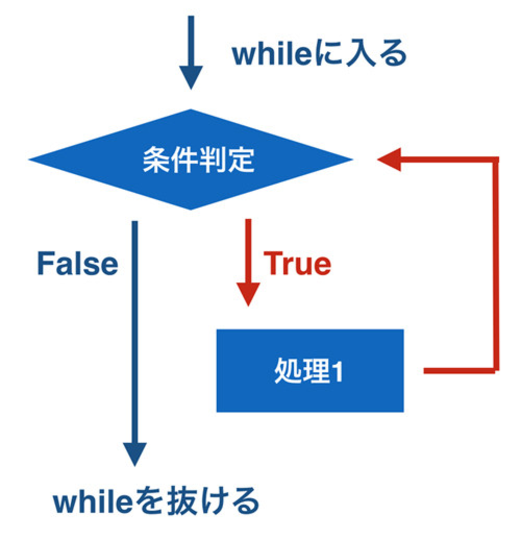
\includegraphics[width=9cm]{003.pdf}
  \caption{Pythonのwhile文}
  \label{scale}
\end{figure}

\begin{lstlisting}[caption=whileの使い方, label=while]
>>> n = 0
>>> while n < 10:
...	 print n
...	 n += 1
\end{lstlisting}
% +=の説明

\subsection{for}
forはリストに格納されている要素をすべてチェックするような処理でよく使われる.range関数を使うことによって指定した回数だけ繰り返し処理を行うことも可能である(ソースコード\ref{for}).
\begin{figure}[h]
 \centering
  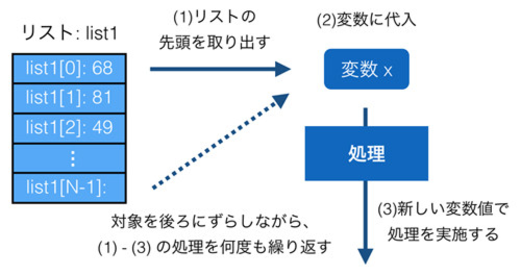
\includegraphics[width=12cm]{002.pdf}
  \caption{Pythonのfor文}
\end{figure}

\begin{lstlisting}[caption=forの使い方, label=for]
>>> n = [1,2,3]
>>> for x in n:
...	print x 	
...
1
2
3
>>> for m in range(10):
...	 print m
...
0
1
2
3
4
5
6
7
8
9
\end{lstlisting}

\newpage
\subsection{break}
whileやforを使った繰り返し処理はbreakを使うことで抜け出すことができる(ソースコード\ref{break}).
\begin{lstlisting}[caption=break, label=break]
>>> for x in range(10):
... 	if x == 5:
... 		break
... 	print x
...
0
1
2
3
4
\end{lstlisting}
%whileを用いて1から1000までの数の和を求めるプログラムを作成せよ


\section{関数}
Pythonには様々な組み込み関数が用意されている.これまで使用してきたrange()やsum(),len()などがそれである.関数を使用する利点としてプログラムの可読性が向上することがあげられる.例えば絶対値を得ようと思った場合,以下のようにifを使って条件分岐させることで実現が可能である(ソースコード\ref{abs1}).
\begin{lstlisting}[caption=絶対値に変換するコード, label=abs1]
>>> x = -5
>>> if(x<0):
...     x = -x
...
>>> print x
5
\end{lstlisting}
同じ処理を組み込み関数であるabs()を使って書くと以下のようになる(ソースコード\ref{abs2}) .
\begin{lstlisting}[caption=abs(), label=abs2]
>>> x = abs(-5)
>>> print(x)
5
\end{lstlisting}
関数には同じコードを何度も書かなくてすむといったメリットもある(ソースコード\ref{abs3}).
\begin{lstlisting}[caption=絶対値に変換するコードを使った場合, label=abs3]
>>> x = 5
>>> y = -10
>>> if(x<0):
... 	x = -x
...
>>> if(y<0):
... 	y = -y
...
>>> print x > y 
False
\end{lstlisting}
関数を使って書き直すとこのようになる(ソースコード\ref{abs4}).
\begin{lstlisting}[caption=abs()を使った場合, label=abs4]
>>> x = 5
>>> y = -10
>>> x = abs(x)
>>> y = abs(y)
>>> print x > y
False
\end{lstlisting}
関数は自分で作成することも可能である.関数は入力を受け取り,それを加工して出力する.入力と出力はなくてもかまわず,入力がない場合は関数の宣言の引数をなくし,出力が不要な場合はreturn文をなくす.関数は宣言した引数に対応する箇所に入力値を入れることで呼び出す.引数がない関数に関しては()に何も入れずに,引数を取る場合は()に値を入力する.(ソースコード\ref{def}).
\begin{lstlisting}[caption=関数の作成, label=def]
# 引数がない関数
>>> def my_func1():
...	 return 0
...
# 返り値がない関数
>>> def my_func2(x):
...	 x = -x
...  
>>> print my_func1()
0
>>> print my_func2(5)
None
\end{lstlisting}
引数は複数指定できるが,return文は一度しか実行されない.
\begin{lstlisting}[caption=returnの動作, label=return]
>>> def my_func3(x, y):
...     print "A"
...     if(x > y):
...         return x
...     print "B"
...     return y
...
>>> print my_func3(5,1)
A
5
>>> print my_func3(2,4)
A
B
4
\end{lstlisting}
上記のソースコード\ref{return}では二つのreturn文が確認できる.x \textgreater yの条件が満たされた場合Bが出力されていないことに注目して欲しい.returnはいくつあっても構わないが,returnされたあとの関数の処理は一切無視される.


\section{スコープ}
スコープとは,ある変数や関数が特定の名前で参照される範囲のことである.ある範囲の外に置いた変数等は,通常,その名前だけでは参照できない.このときこれらの変数はスコープ外であると言われる.プログラミングでは,予期しない誤作動を避けるためにも,それぞれの作業段階で必要のない名前はできるだけ参照されないようにすることが望ましい.


Pythonではif文やfor文などの制御構造はスコープを作らない.つまり,if文やfor文の中で宣言された変数は,if文やfor文のブロックの外からも参照することができる.しかし,関数定義とクラス定義では新しいスコープが作られる.つまり,関数定義の内側と外側に同じ名前の変数が存在しても,両者は区別される.


\begin{lstlisting}[caption=スコープ,label=scope]
>>> x = 5 #一番外側のスコープで変数xに5を代入
>>> def scope_test(): #scope_test関数の定義
...     x = 10 #関数定義のブロック内でxに10を代入
...     print x #変数xの値を出力
... #関数定義のブロックを抜けるためにEnter
>>> print x #変数xの値を出力
5
>>> scope_test() #scope_test関数の実行
10
\end{lstlisting}